\subsection{Set Notation and Common Sets}

\begin{defn}[Set]\index{set}
    A set is a finite or infinite collection of objects in which order has no significance, and multiplicity is generally also ignored (unlike a list or multiset). Members of a set are often referred to as elements and the notation a in A is used to denote that a is an element of a set A. The study of sets and their properties is the object of set theory.\cite{mathworldset}
\end{defn}

\begin{note}[Common Sets]
    Here are six sets that we will frequently use:
    \begin{enumerate}
        \item \emph{Empty Set}: \(\emptyset=\{\}\),
        \item \emph{Natural Numbers}: \[\bbN=\left\{1,2,3,\ldots\right\},\]
        \item \emph{Integers}: \[\bbZ=\left\{0,\pm1,\pm2,\pm3,\ldots\right\},\]
        \item \emph{Rational Numbers}: \[\bbQ=\left\{a/b\middle|a,b\in\bbZ \wedge b\neq0\right\},\]
        \item \emph{Real Numbers}: \[\bbR=\bbQ\cup \left\{irrationals\right\}\] or all the numbers used to denote or measure distances on a line, and
        \item \emph{Complex Numbers}: \[\bbC=\left\{a+bi\middle|a,b\in\bbR \wedge i^2=-1\right\}.\]
    \end{enumerate}\index{natural numbers}\index{rational numbers}\index{real numbers}\index{complex numbers}\index{complex numbers}\index{empty set}
\end{note}


% Set Roster Set Builder
\begin{defn}[Set Notations]\index{set roster notation}\index{set builder notation}
    Describing a set by listing its elements is called \emph{set roster} notation:
    \begin{equation}\label{eq:set_roster}
        S=\left\{2,4,6,8,10,12,14,16,18\right\}.
    \end{equation}
    Describing a set by setting conditions for membership is called \emph{set builder} notation:
    \begin{equation}\label{eq:set_builder}
        S=\left\{2n\middle| n\ is\ an\ integer\ and\ 0<n<10\right\}.
    \end{equation}
    Either way this could be read as 
    \begin{quote}
        The set of all integers of the form \(2n\) with \(n\) from 1 to 9,
    \end{quote}
    or in plainer language
    \begin{quote}
        All the even integers from two to eighteen.
    \end{quote}

    To read the sets in set builder notation we need to note some new-ish notation:
    \begin{figure}[H]
        \centering
        % \inputtikz{setbuilder}
        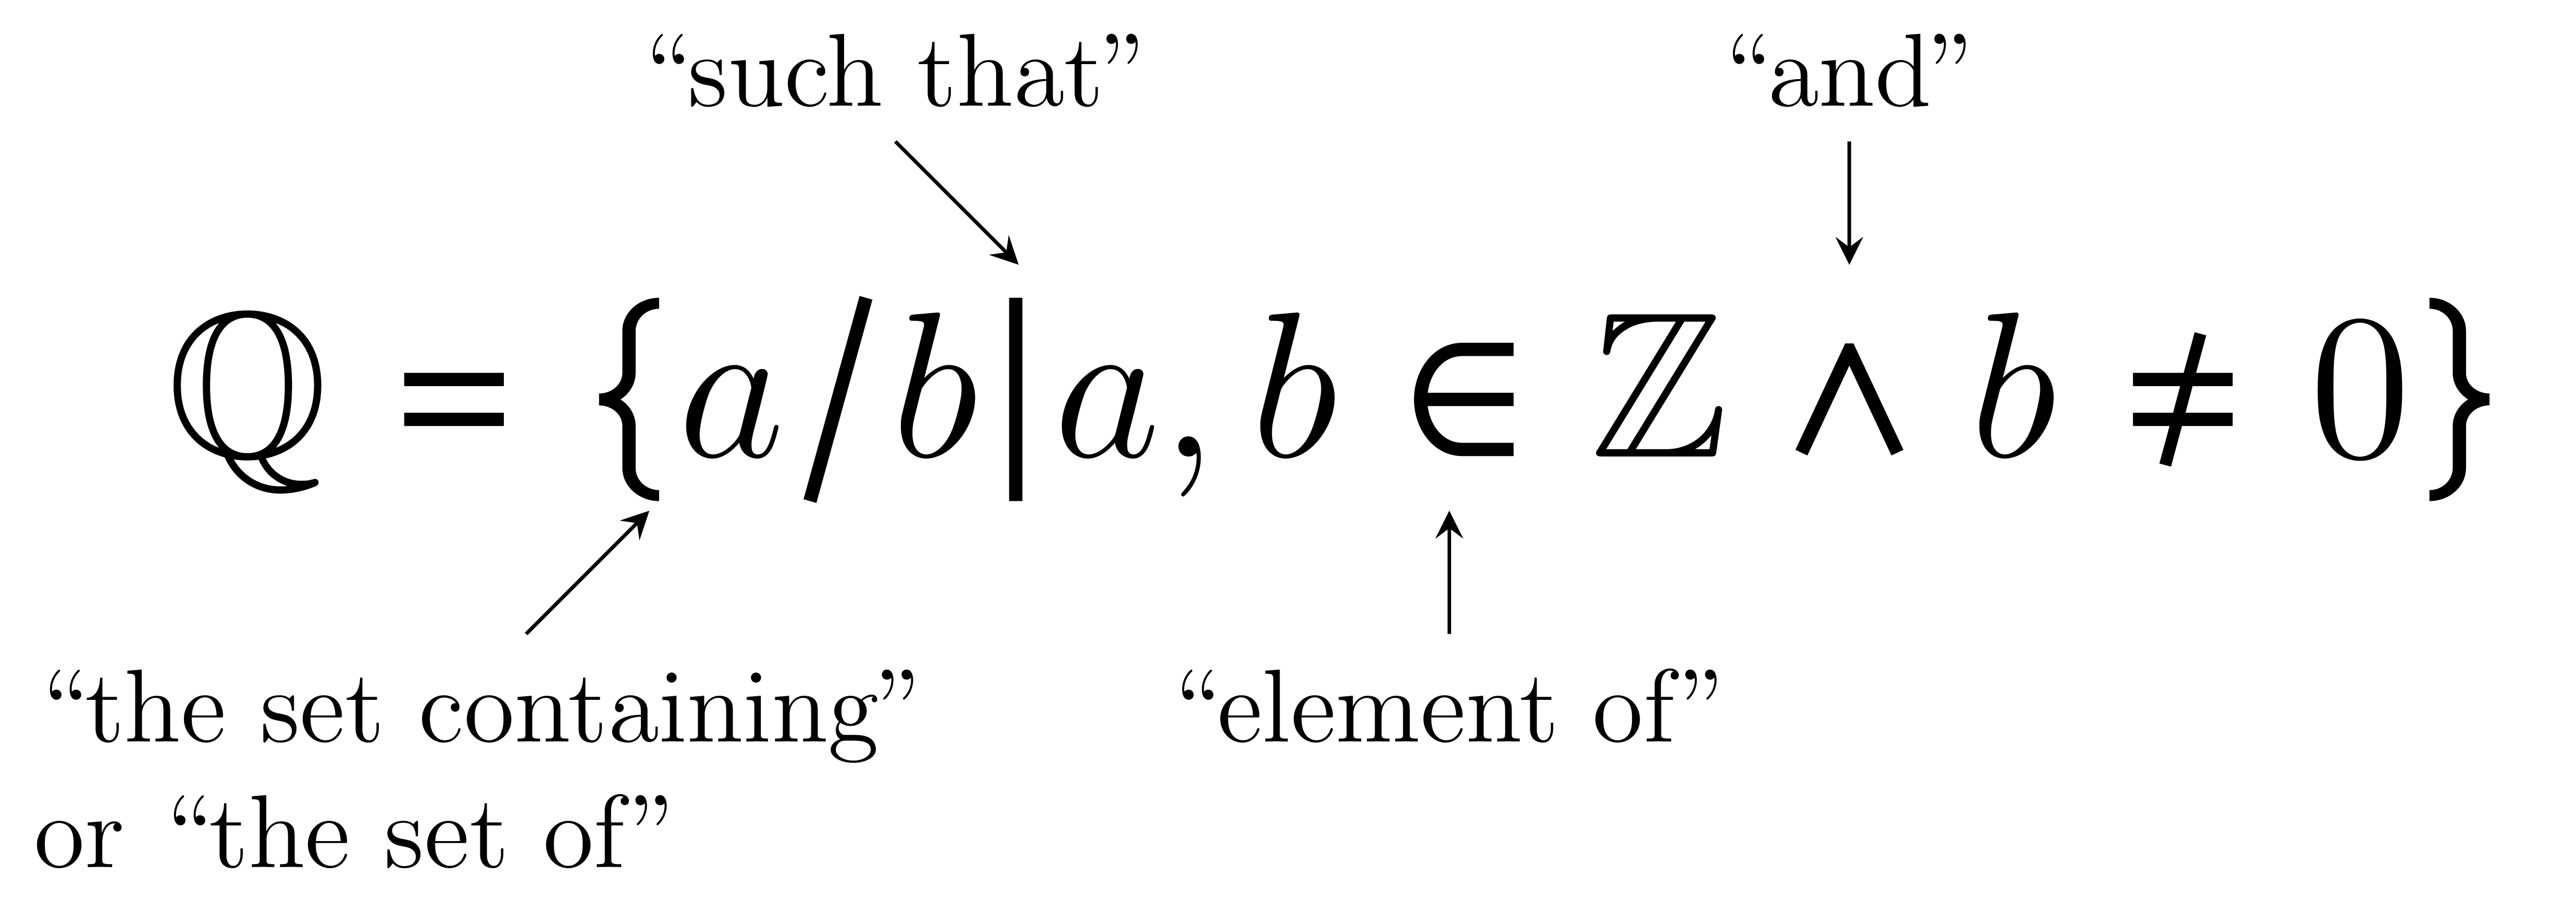
\includegraphics[scale=0.06,alt={Diagram describing components of set builder notation},width=0.55\linewidth]{images/created/setbuilder.png}
        \caption{Set Builder Notation}
        \label{fig:setbuilder}
    \end{figure}
    So we can translate the description of the rationals as
    \begin{quote}
        The rational numbers are \emph{the set of} all ratios \(a/b\) \emph{such that} \(a\) and \(b\) are \emph{elements of} the integers \emph{and} \(b\) does not equal 0.
    \end{quote}   
\end{defn}

% Converting Between Them
\begin{practiceprob}
    Given the set \(A=\left\{1/2,2/2,3/2,4/2,5/2,\ldots \right\}\) write the set as a sentence and then in set builder notation.

    Verbal/Written Description:
    {\large
    \begin{quote}
        The set \(A\) is the set of 
    \end{quote}
    }
    \vspace{1\baselineskip}

    Set Builder Description:
    {\Large
        \[A=\left\{\phantom{\rule{70pt}{30pt}}\middle|\phantom{\rule{140pt}{30pt}}\right\}\]
    }
\end{practiceprob}

\begin{practiceprob}
    Given the set \(B=\left\{n^2/5\middle|n\in\bbZ\right\}\) write the set as a sentence and then in set roster notation.

    Verbal/Written Description:
    {\large
    \begin{quote}
        The set \(B\) is the set of 
    \end{quote}
    }
    \vspace{1\baselineskip}

    Set Roster Description:
    {\Large
        \[B=\left\{\phantom{\rule{210pt}{30pt}}\right\}\]
    }
\end{practiceprob}

\begin{practiceprob}
    The set \(C\) is the set of all odd natural numbers less than 30, write the set in set roster notation and then in set builder notation.

    Set Roster Description:
    {\Large
        \[C=\left\{\phantom{\rule{0.7\textwidth}{30pt}}\right\}\]
    }


    Set Builder Description:
    {\Large
        \[C=\left\{\phantom{\rule{70pt}{30pt}}\middle|\phantom{\rule{140pt}{30pt}}\right\}\]
    }
\end{practiceprob}

\clearpage

\subsection{New Sets From Old}
% Union, Intersection, Difference
\begin{defn}[Basic Set Combinations]\index{union}\index{intersection}\index{set difference}
    Given sets \(A=\left\{1,3,5,7,9\right\}\) and \(B=\left\{2,3,5,7\right\}\):
    \begin{itemize}
        \item \emph{Union of \(A\) and \(B\)}:
        \begin{equation}\label{eq:union}
            A\cup B=\left\{x\middle|x\in A\ \vee x\in B \right\} = \left\{1,2,3,5,7,9\right\}
        \end{equation}
        \item \emph{Intersection of \(A\) and \(B\)}:
        \begin{equation}\label{eq:intersection}
            A\cap B=\left\{x\middle|x\in A\ \wedge x\in B \right\} = \left\{3,5,7\right\}
        \end{equation}
        \item \emph{Difference between \(A\) and \(B\)}:
        \begin{equation}\label{eq:difference}
            A\setminus B=\left\{x\middle|x\in A\ \wedge x\not\in B \right\} = \left\{1,9\right\}
        \end{equation}
    \end{itemize}
\end{defn}

\begin{practiceprob}
    Given \(C=\left\{n\middle|n\in\bbZ\wedge -5\leq n\leq5\right\}\) and\newline \(D=\left\{-2,-3,-5,-7,-11,-13,-17,-19\right\}\) find the following:
        \begin{itemize}
            \item \(C\cup D=\left\{\phantom{\rule{280pt}{18pt}}\right\}\)
            \item \(C\cap D=\left\{\phantom{\rule{280pt}{18pt}}\right\}\)
            \item \(C\setminus D=\left\{\phantom{\rule{280pt}{18pt}}\right\}\)
            \item \(D\setminus C=\left\{\phantom{\rule{280pt}{18pt}}\right\}\)
        \end{itemize}
\end{practiceprob}
\begin{practiceprob}
    Given \(V=\left\{a,e,i,o,u,y\right\}\) of vowels and\newline \(C=\left\{b,c,d,f,g,h,j,k,l,m,n,p,q,r,s,t,v,w,x,y,z\right\}\) of consonants find the following:
        \begin{itemize}
            \item \(V\cup C=\left\{\phantom{\rule{280pt}{18pt}}\right\}\)
            \item \(V\cap C=\left\{\phantom{\rule{280pt}{18pt}}\right\}\)
            \item \(C\setminus V=\left\{\phantom{\rule{280pt}{18pt}}\right\}\)
            \item \(V\setminus C=\left\{\phantom{\rule{280pt}{18pt}}\right\}\)
        \end{itemize}
\end{practiceprob}

\clearpage

% Universal Sets and Complements
\begin{exposition}[Universal Sets, Compliments, and Visualization]\index{universal set}\index{set complement}\index{subset}\index{Venn diagram}
    Again letting \(A=\left\{1,3,5,7,9\right\}\) and \(B=\left\{2,3,5,7\right\}\) we could let 
    \[
        \mathscr{U}=\left\{n\middle| n\in\bbN\wedge n\leq 10\right\}=\left\{1,2,3,4,5,6,7,8,9,10\right\}
    \]
    be the \emph{universal set} from which \(A\) and \(B\) draw elements so we can now write \[A=\left\{x\middle|x\in\mathscr{U}\wedge x\ is\ odd\right\}\ \text{and}\ B=\left\{x\middle|x\in\mathscr{U}\wedge x\ is\ prime\right\}.\]  And we say \(A\) and \(B\) are \emph{subsets}\footnote{Or that \(\mathscr{U}\) is a superset of \(A\) and \(B\).} of \(\mathscr{U}\).  We can also now define the \emph{compliment} of a set \(A\) as
    \begin{equation}\label{eq:compliment}
        A^c=\left\{x\middle|x\in\mathscr{U}\wedge x\not\in A\right\}=\left\{2,4,6,8,10\right\}.
        \footnote{Some texts us the notation \(\overline{A}\) for the compliment of \(A\).}
    \end{equation}
    Finally we can picture all of this with a \emph{Venn Diagram}:
    \begin{figure}[H]
        \centering
        % \inputtikz{twosetvenn}
        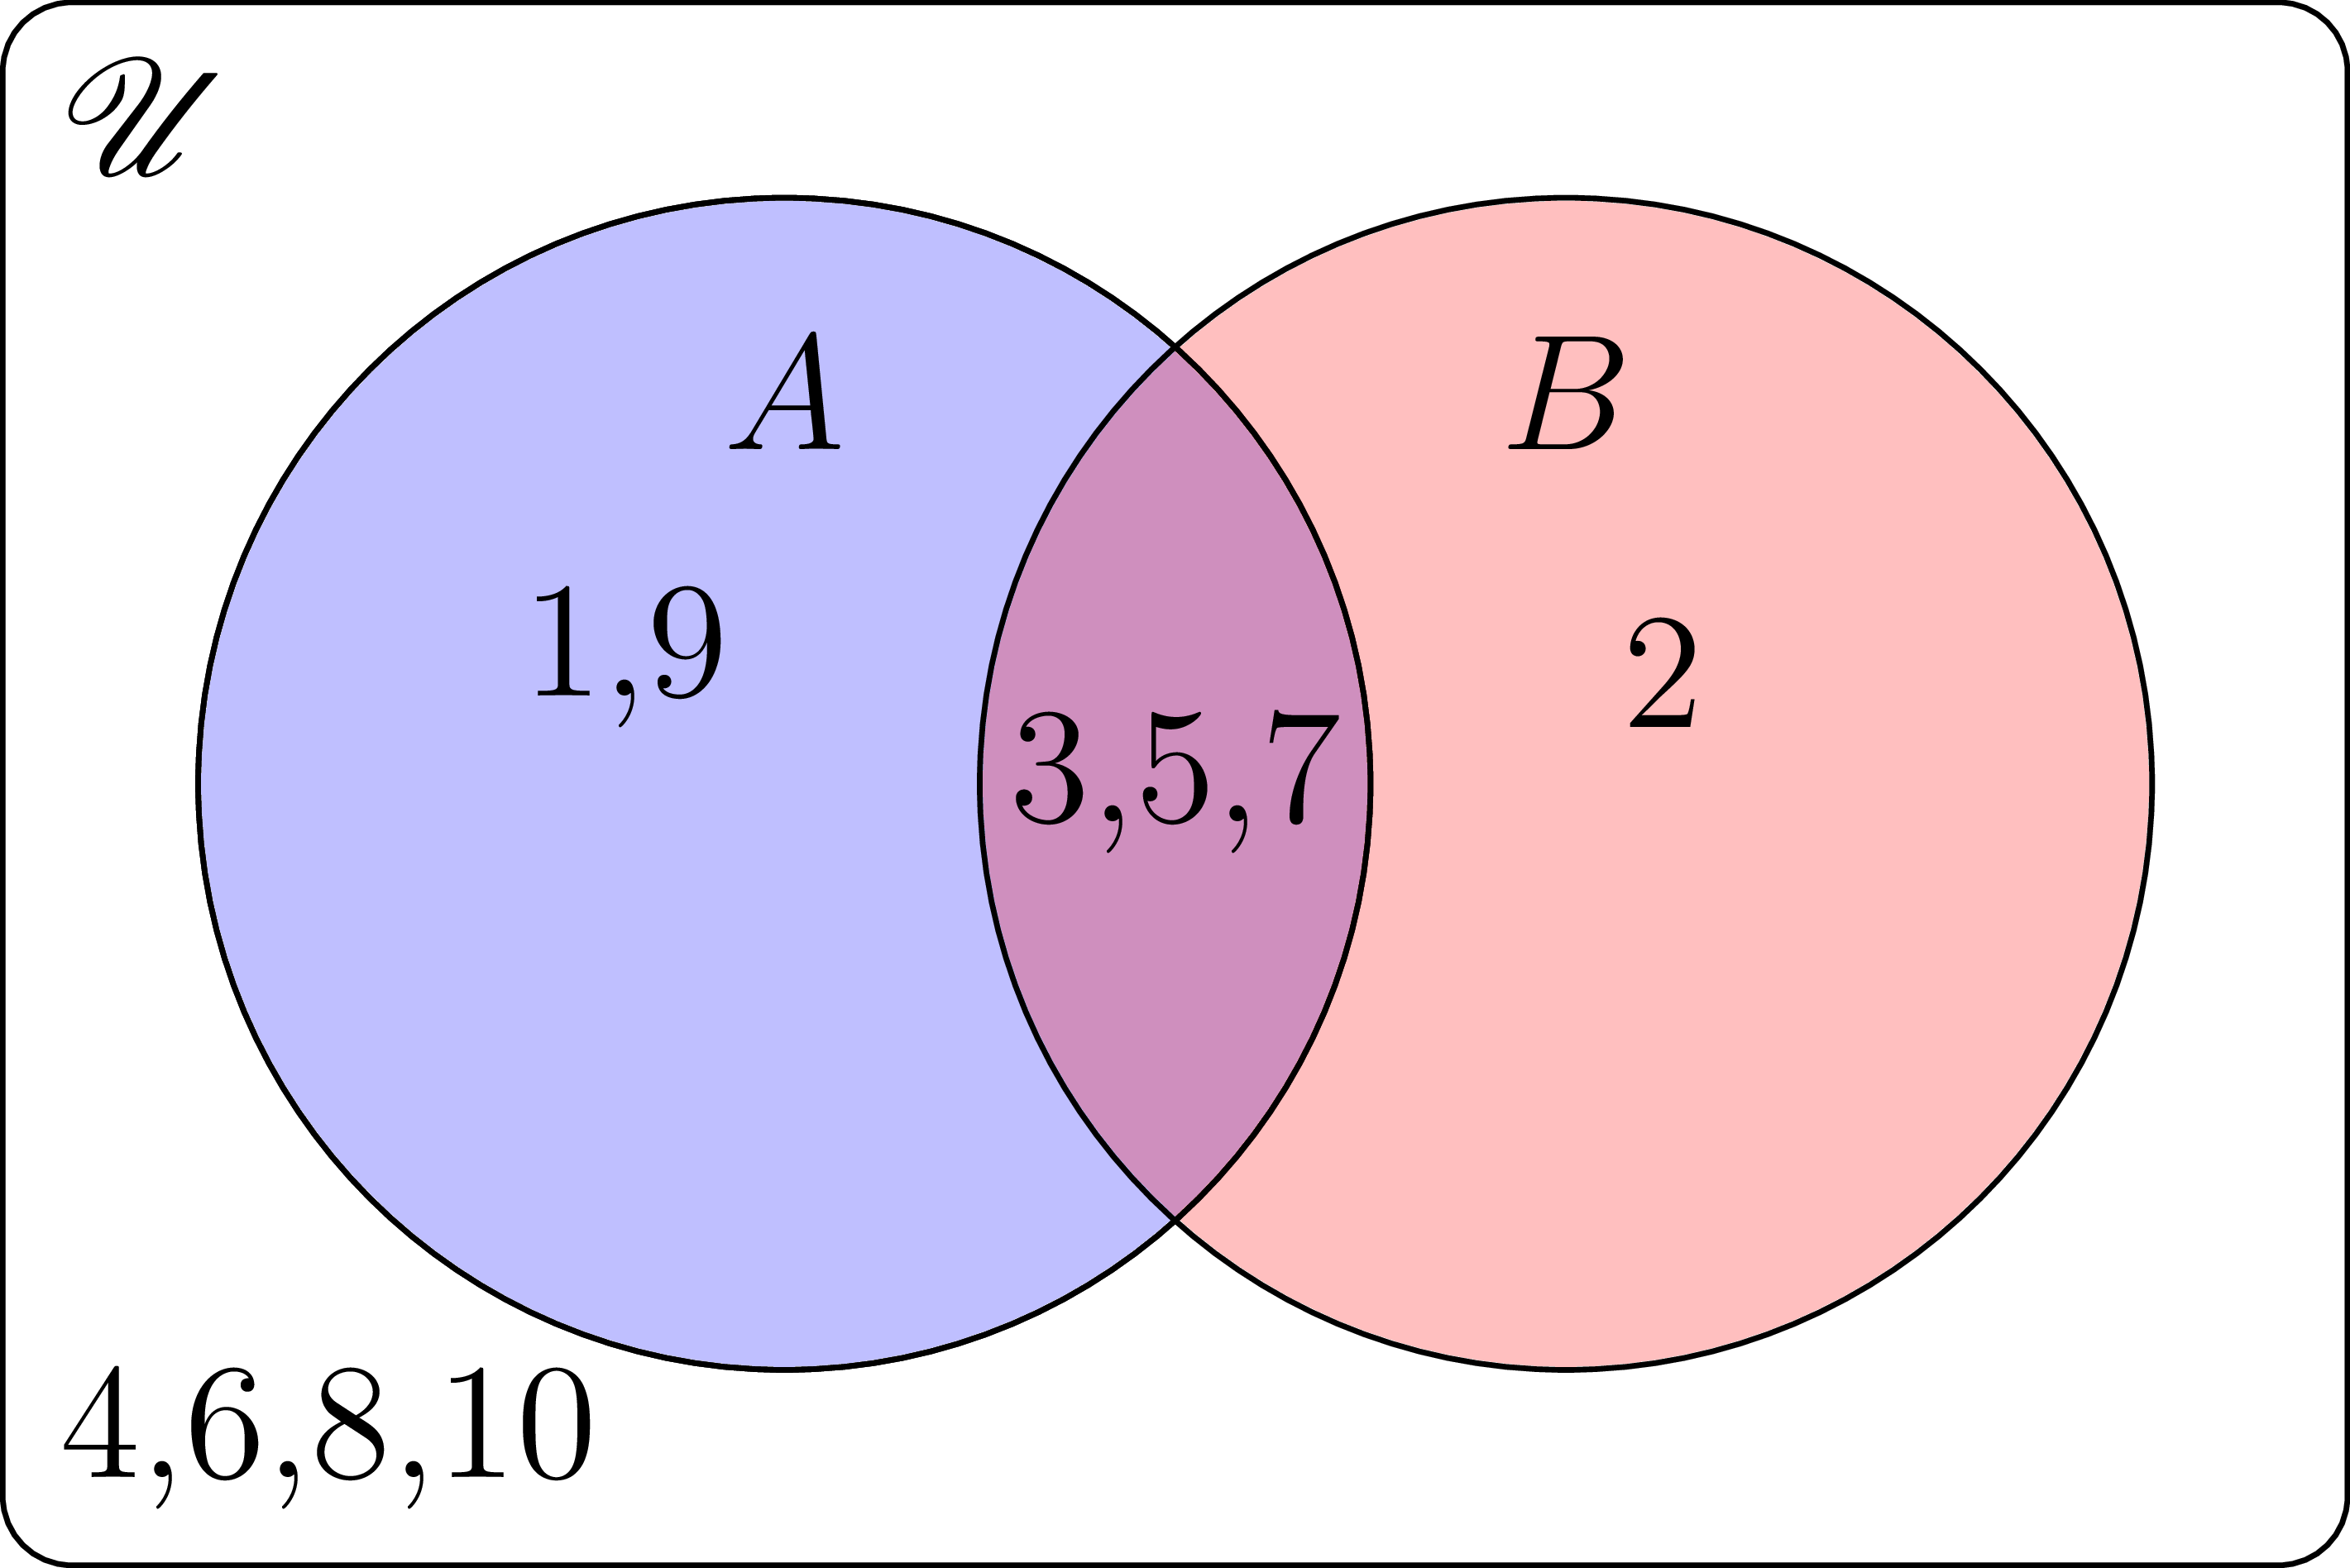
\includegraphics[scale=0.06,alt={Venn diagram of sets A and B listed above.},width=0.33\linewidth]{images/created/twosetvenn.png}
        \caption{Venn Diagram for Sets \(A\) and \(B\)}
        \label{fig:abvenndiagram}
    \end{figure}
\end{exposition}


\begin{practiceprob}   Use the Venn diagram to help you fill in the following sets.

\begin{sides}[lefthand width=0.5\textwidth]
    \begin{align*}
        \mathscr{U} &= \left\{\phantom{\rule{0.6\textwidth}{15pt}}\right\}\\
        C &= \left\{\phantom{\rule{0.6\textwidth}{15pt}}\right\}\\
        C^c &= \left\{\phantom{\rule{0.6\textwidth}{15pt}}\right\}\\
        A\cap C^c &= \left\{\phantom{\rule{0.6\textwidth}{15pt}}\right\}\\
        A^c \cap B\cap C &= \left\{\phantom{\rule{0.6\textwidth}{15pt}}\right\}\\
        A\cup B^c\cup C^c &= \left\{\phantom{\rule{0.6\textwidth}{15pt}}\right\}
    \end{align*}
    \tcblower
    \begin{figure}[H]
        \centering
        % \inputtikz{threesetvenndiagram}
        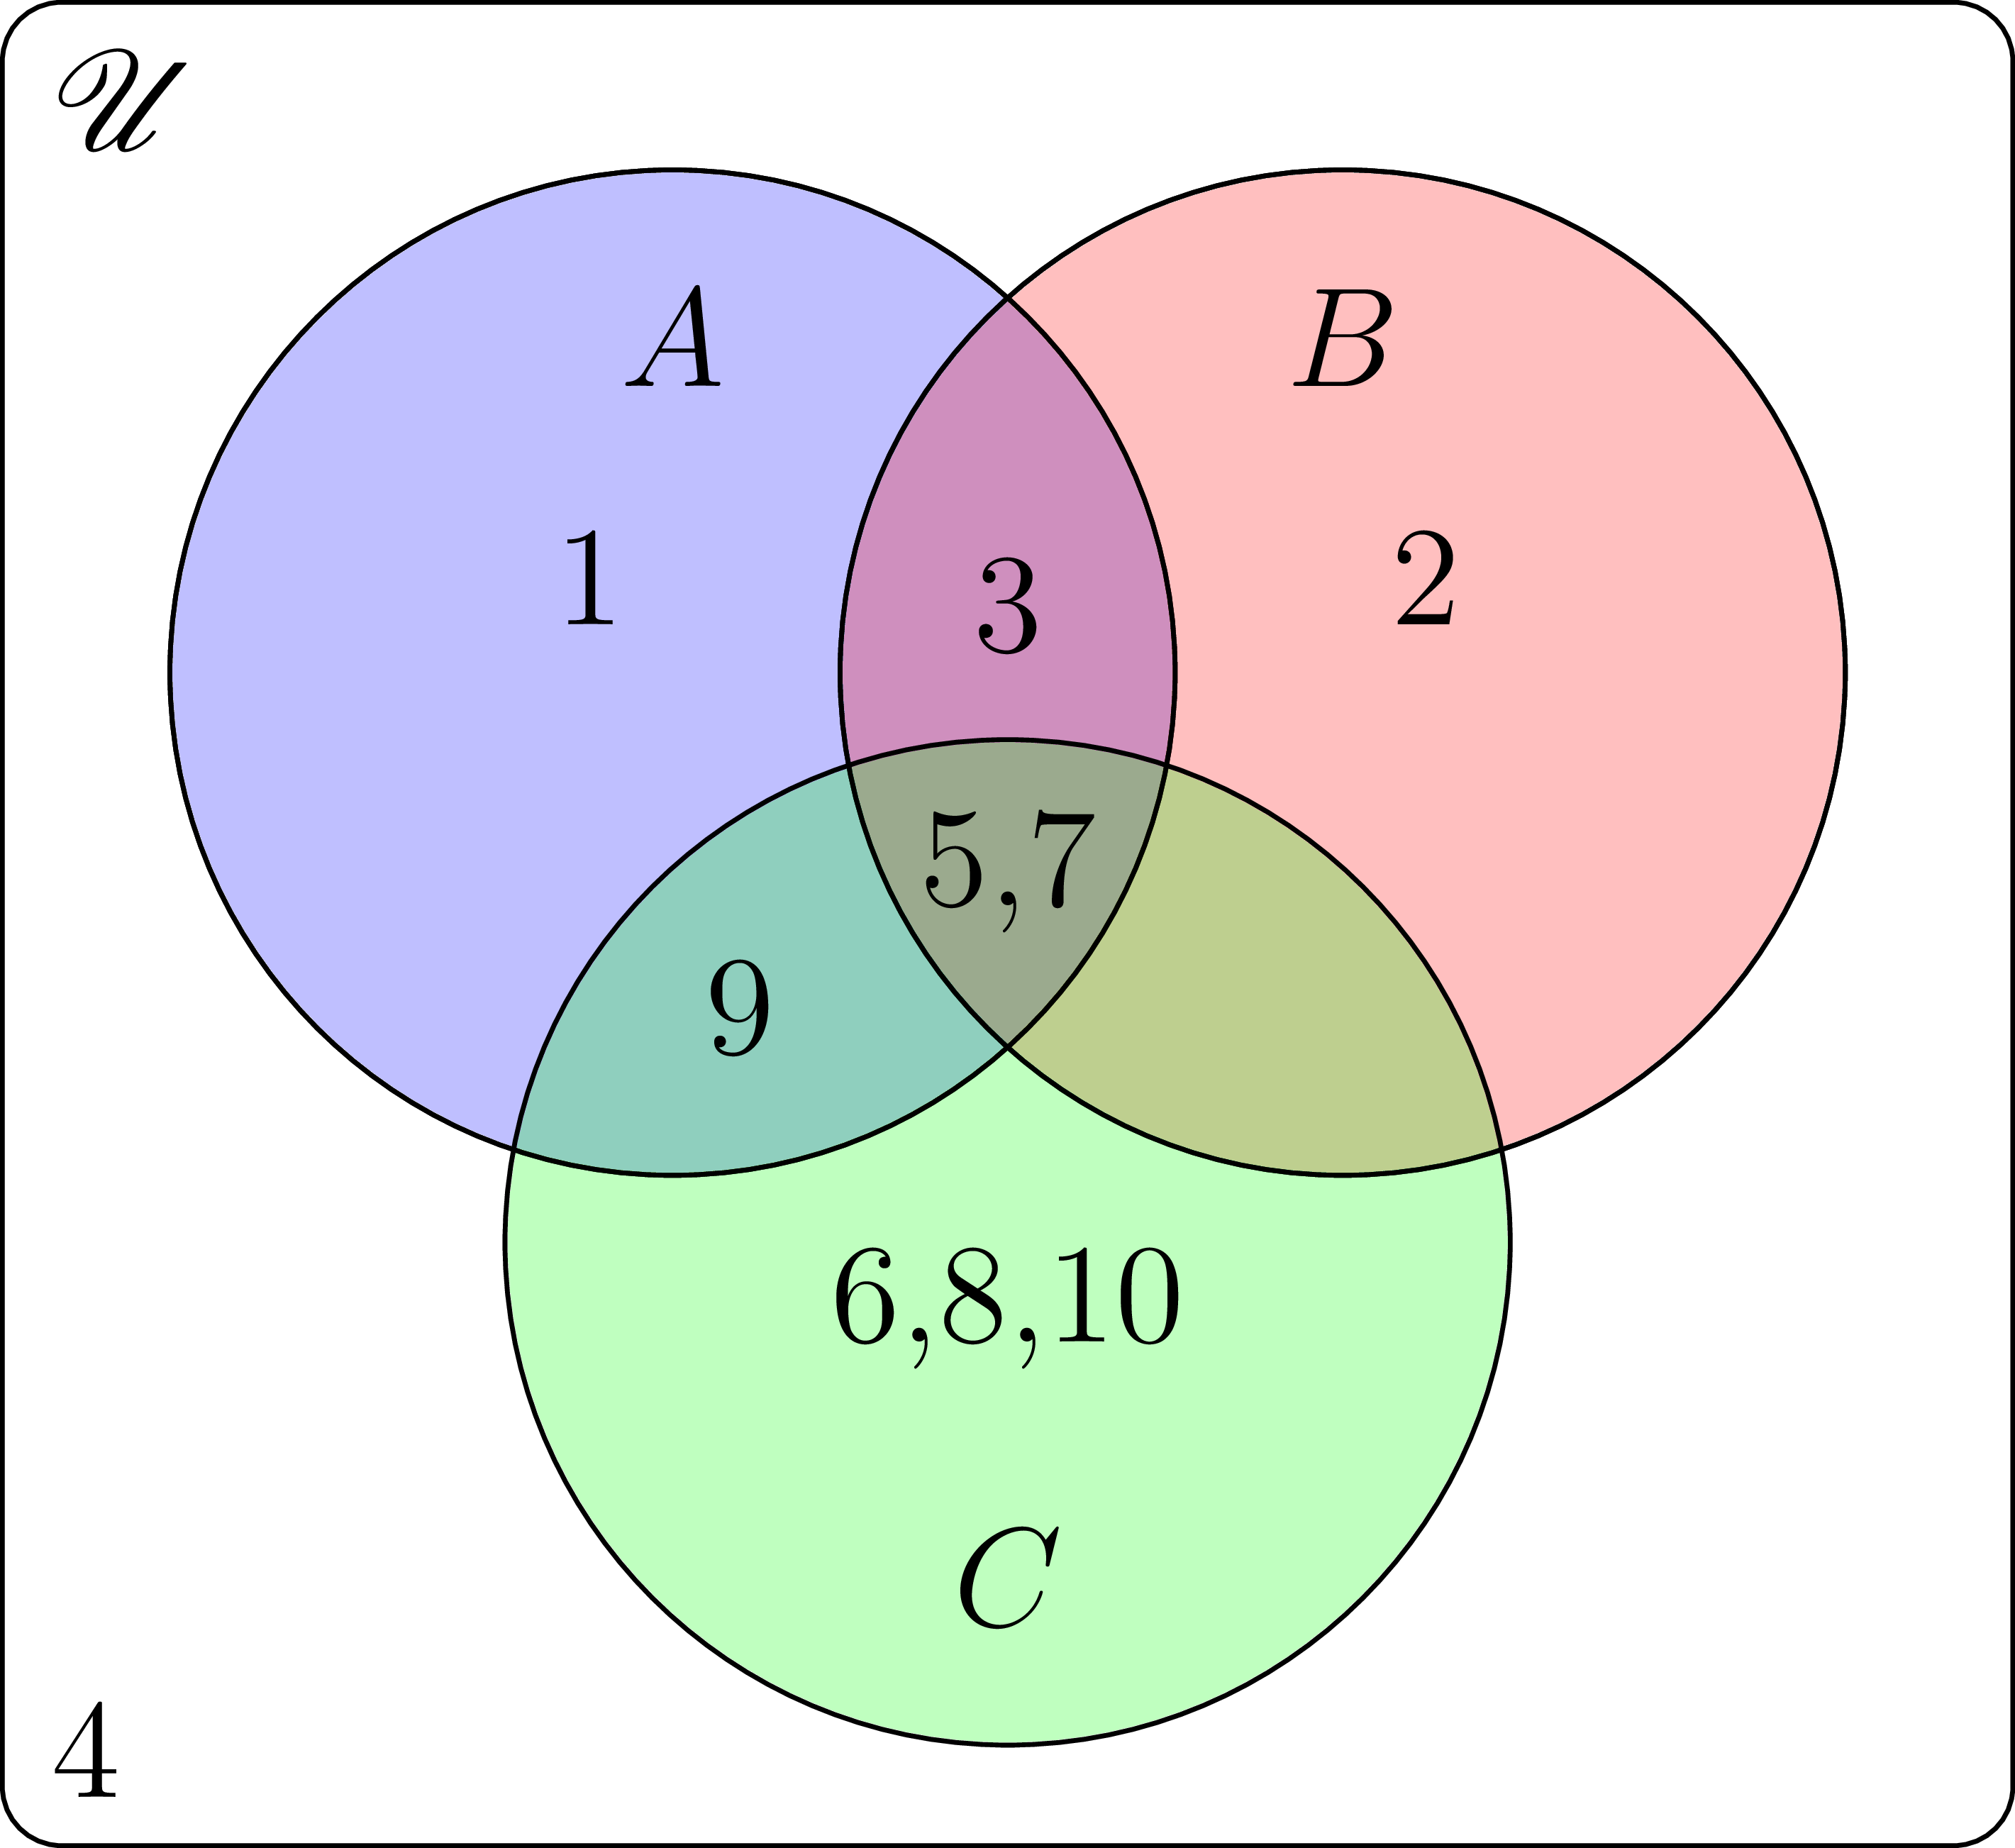
\includegraphics[width=0.73\linewidth,alt={Venn diagram with three sets A, B, and C}]{images/created/threesetvenndiagram.png}
        \caption{Venn Diagram with Sets \(A\), \(B\), and \(C\)}
        \label{fig:threesetvenndiagram}
    \end{figure}
\end{sides}
\end{practiceprob}

\clearpage

\begin{practiceprob}
    Use the Venn diagram to help you match up the following sets.
    
    \begin{align*}
        \rule{15pt}{0.2pt}\ (a)&\ A^c & (1)&\ A^c\cap B \\
        \rule{15pt}{0.2pt}\ (b)&\ B\setminus A & (2)&\ (A^c\cup B^c)^c \\
        \rule{15pt}{0.2pt}\ (c)&\ A\cup B^c & (3)&\ \mathscr{U}\setminus A \\
        \rule{15pt}{0.2pt}\ (d)&\ A\cap B & (4)&\ (A^c\cap B)^c \\ 
        \rule{15pt}{0.2pt}\ (e)&\ (A\cup B)\setminus (A\cap B) & (5)&\ (B\setminus A)\cup (A\setminus B)
    \end{align*}

    \begin{figure}[H]
        \centering
        % \inputtikz{emptytwosetvenn}
        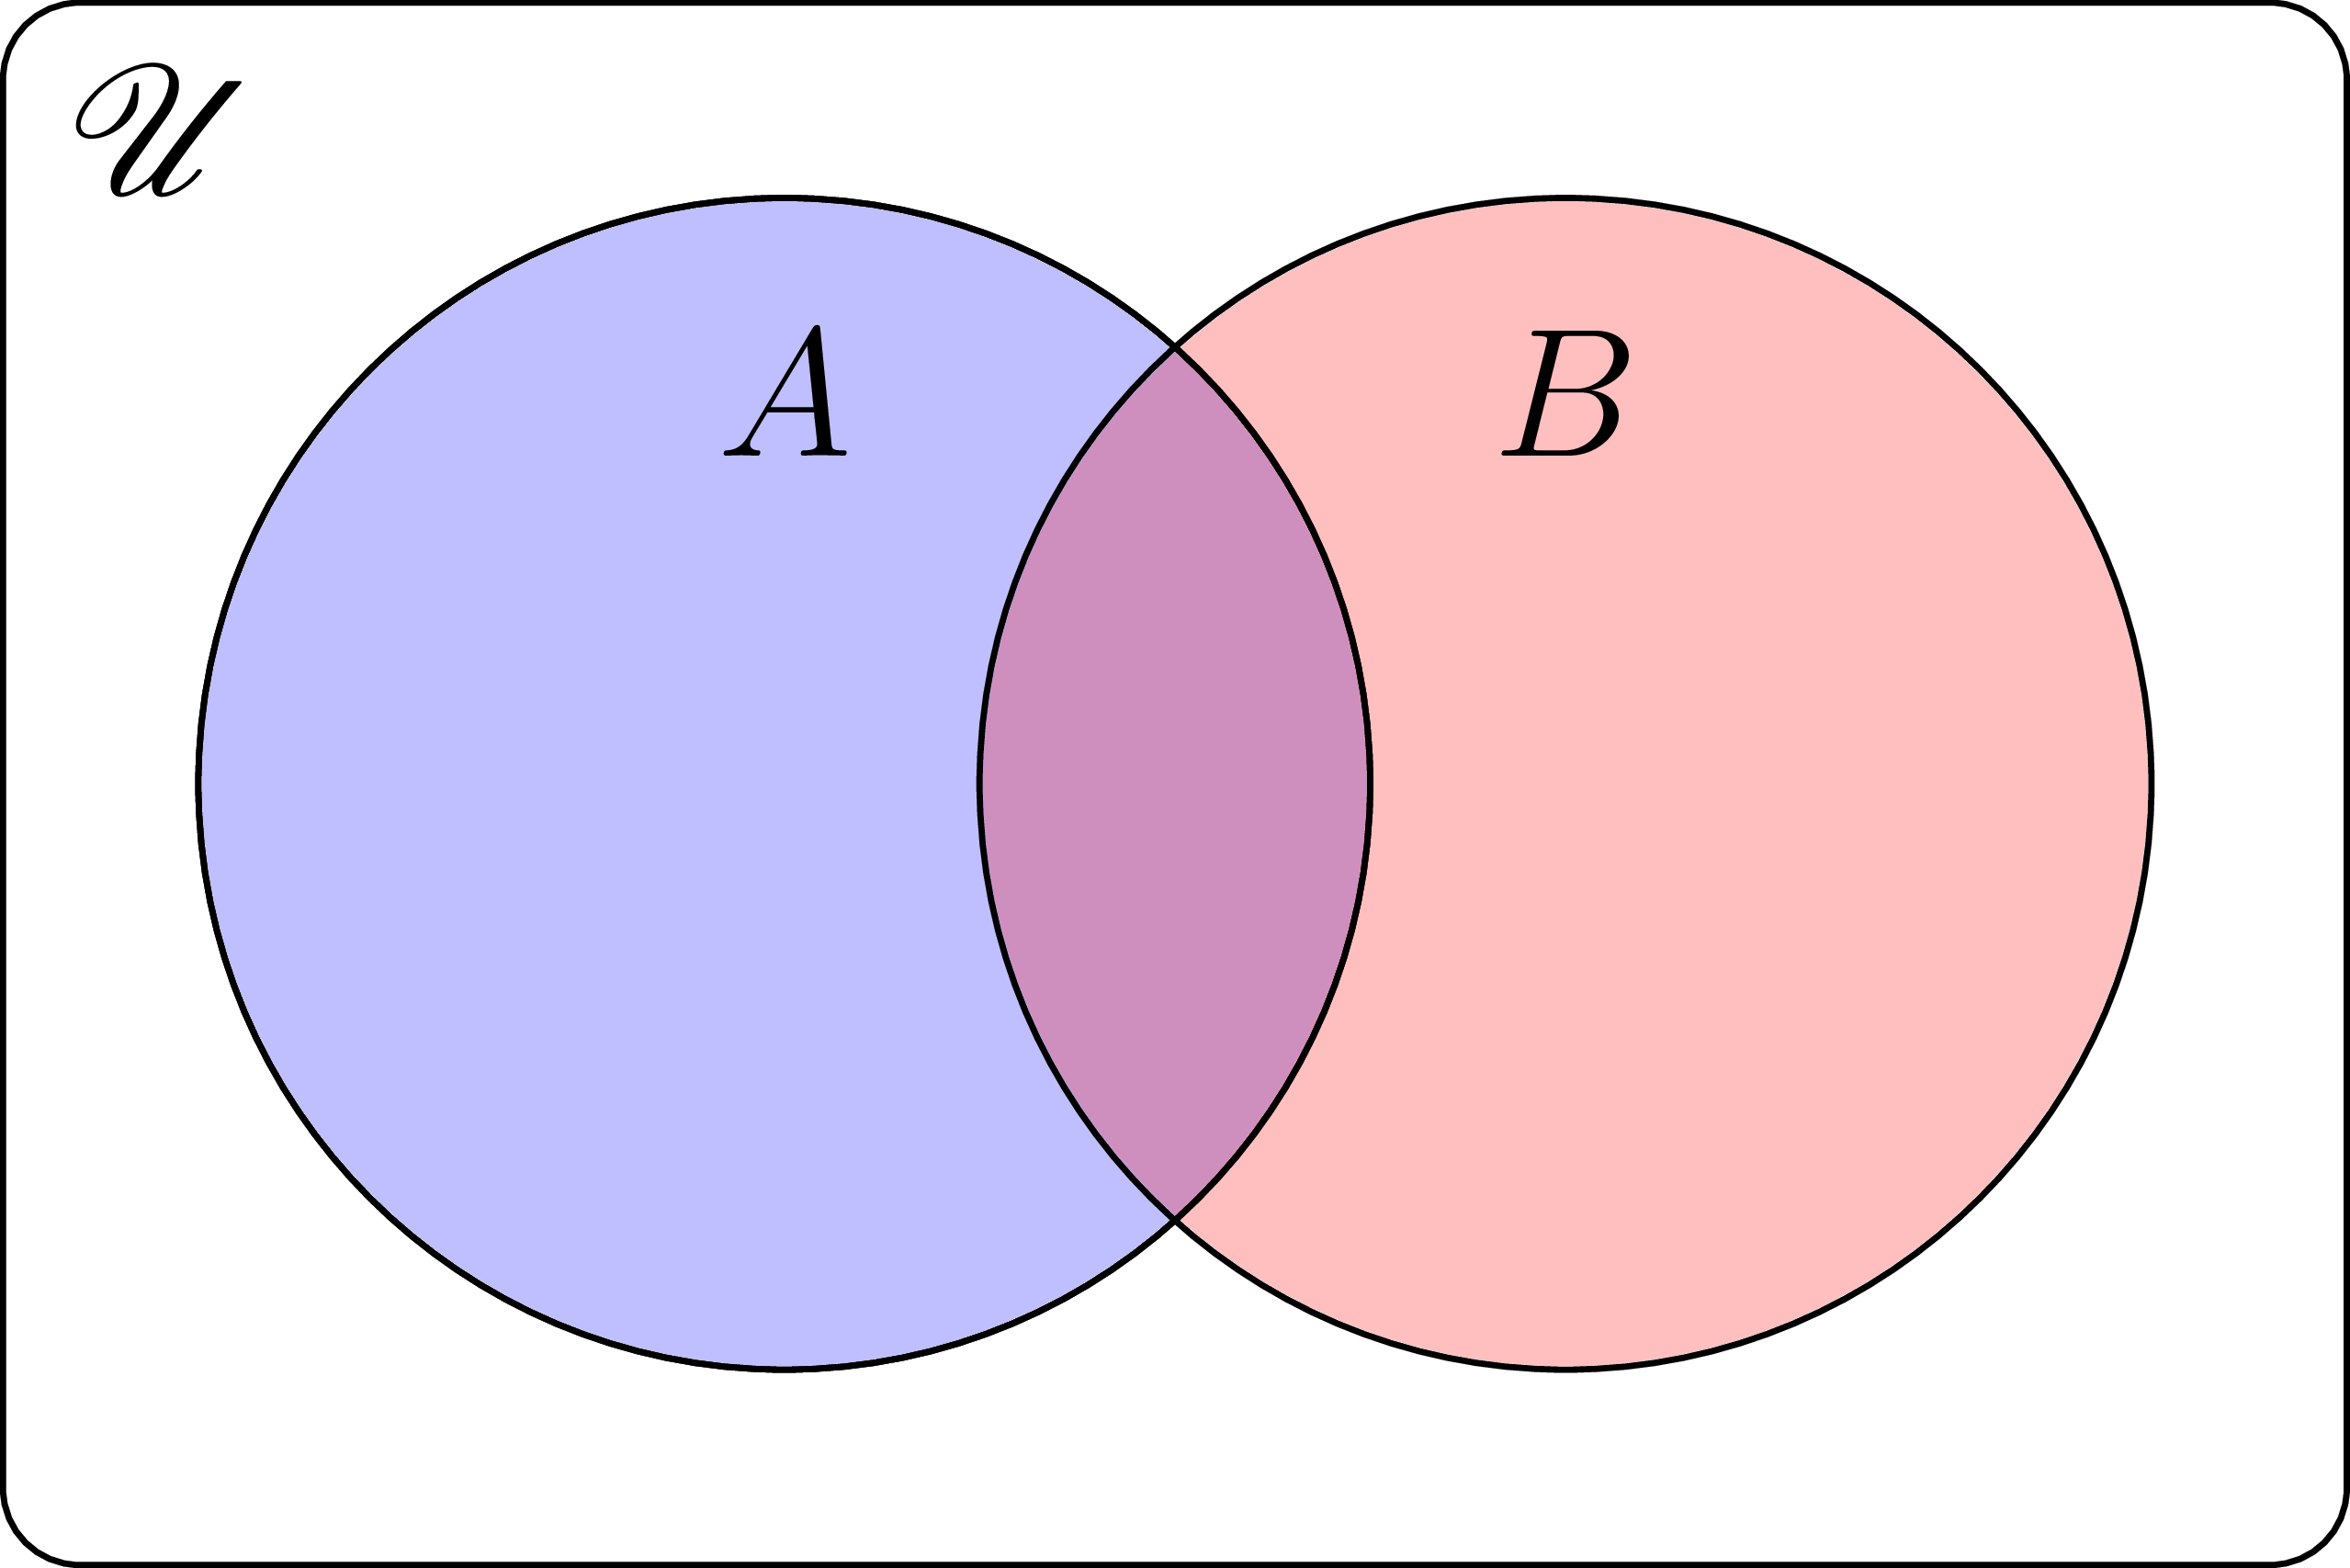
\includegraphics[width=0.35\linewidth,alt={A blank venn diagram with two sets.}]{images/created/emptytwosetvenn.png}
        \caption{Blank Two Set Venn Diagram}
        \label{fig:emptyvenn}
    \end{figure}
\end{practiceprob}


% Product & Power Set
\begin{defn}[Products of Sets]\index{Cartesian product}\index{ordered pair}
    Again letting \(A=\left\{1,3,5,7,9\right\}\) and \(B=\left\{2,3,5,7\right\}\) we can define the \emph{Cartesian Product} of \(A\) and \(B\) as
    \begin{align}\label{eq:product}
        A\times B&=\left\{(a,b)\middle|a\in A\wedge b\in B\right\},\\
            &=\left\{(1,2),(1,3),(1,5),(1,7),(3,2),(3,3),(3,5),(3,7),(5,2),(5,3),\right.\nonumber\\
            &\hspace*{24pt}\left.(5,5),(5,7),(7,2),(7,3),(7,5),(7,7),(9,2),(9,3),(9,5),(9,7)\right\}\nonumber
    \end{align}
    a new set with \emph{ordered pairs} of numbers instead of just individual numbers as elements.
    \begin{figure}[H]
        \centering
        % \inputtikz{cartesianproduct}
        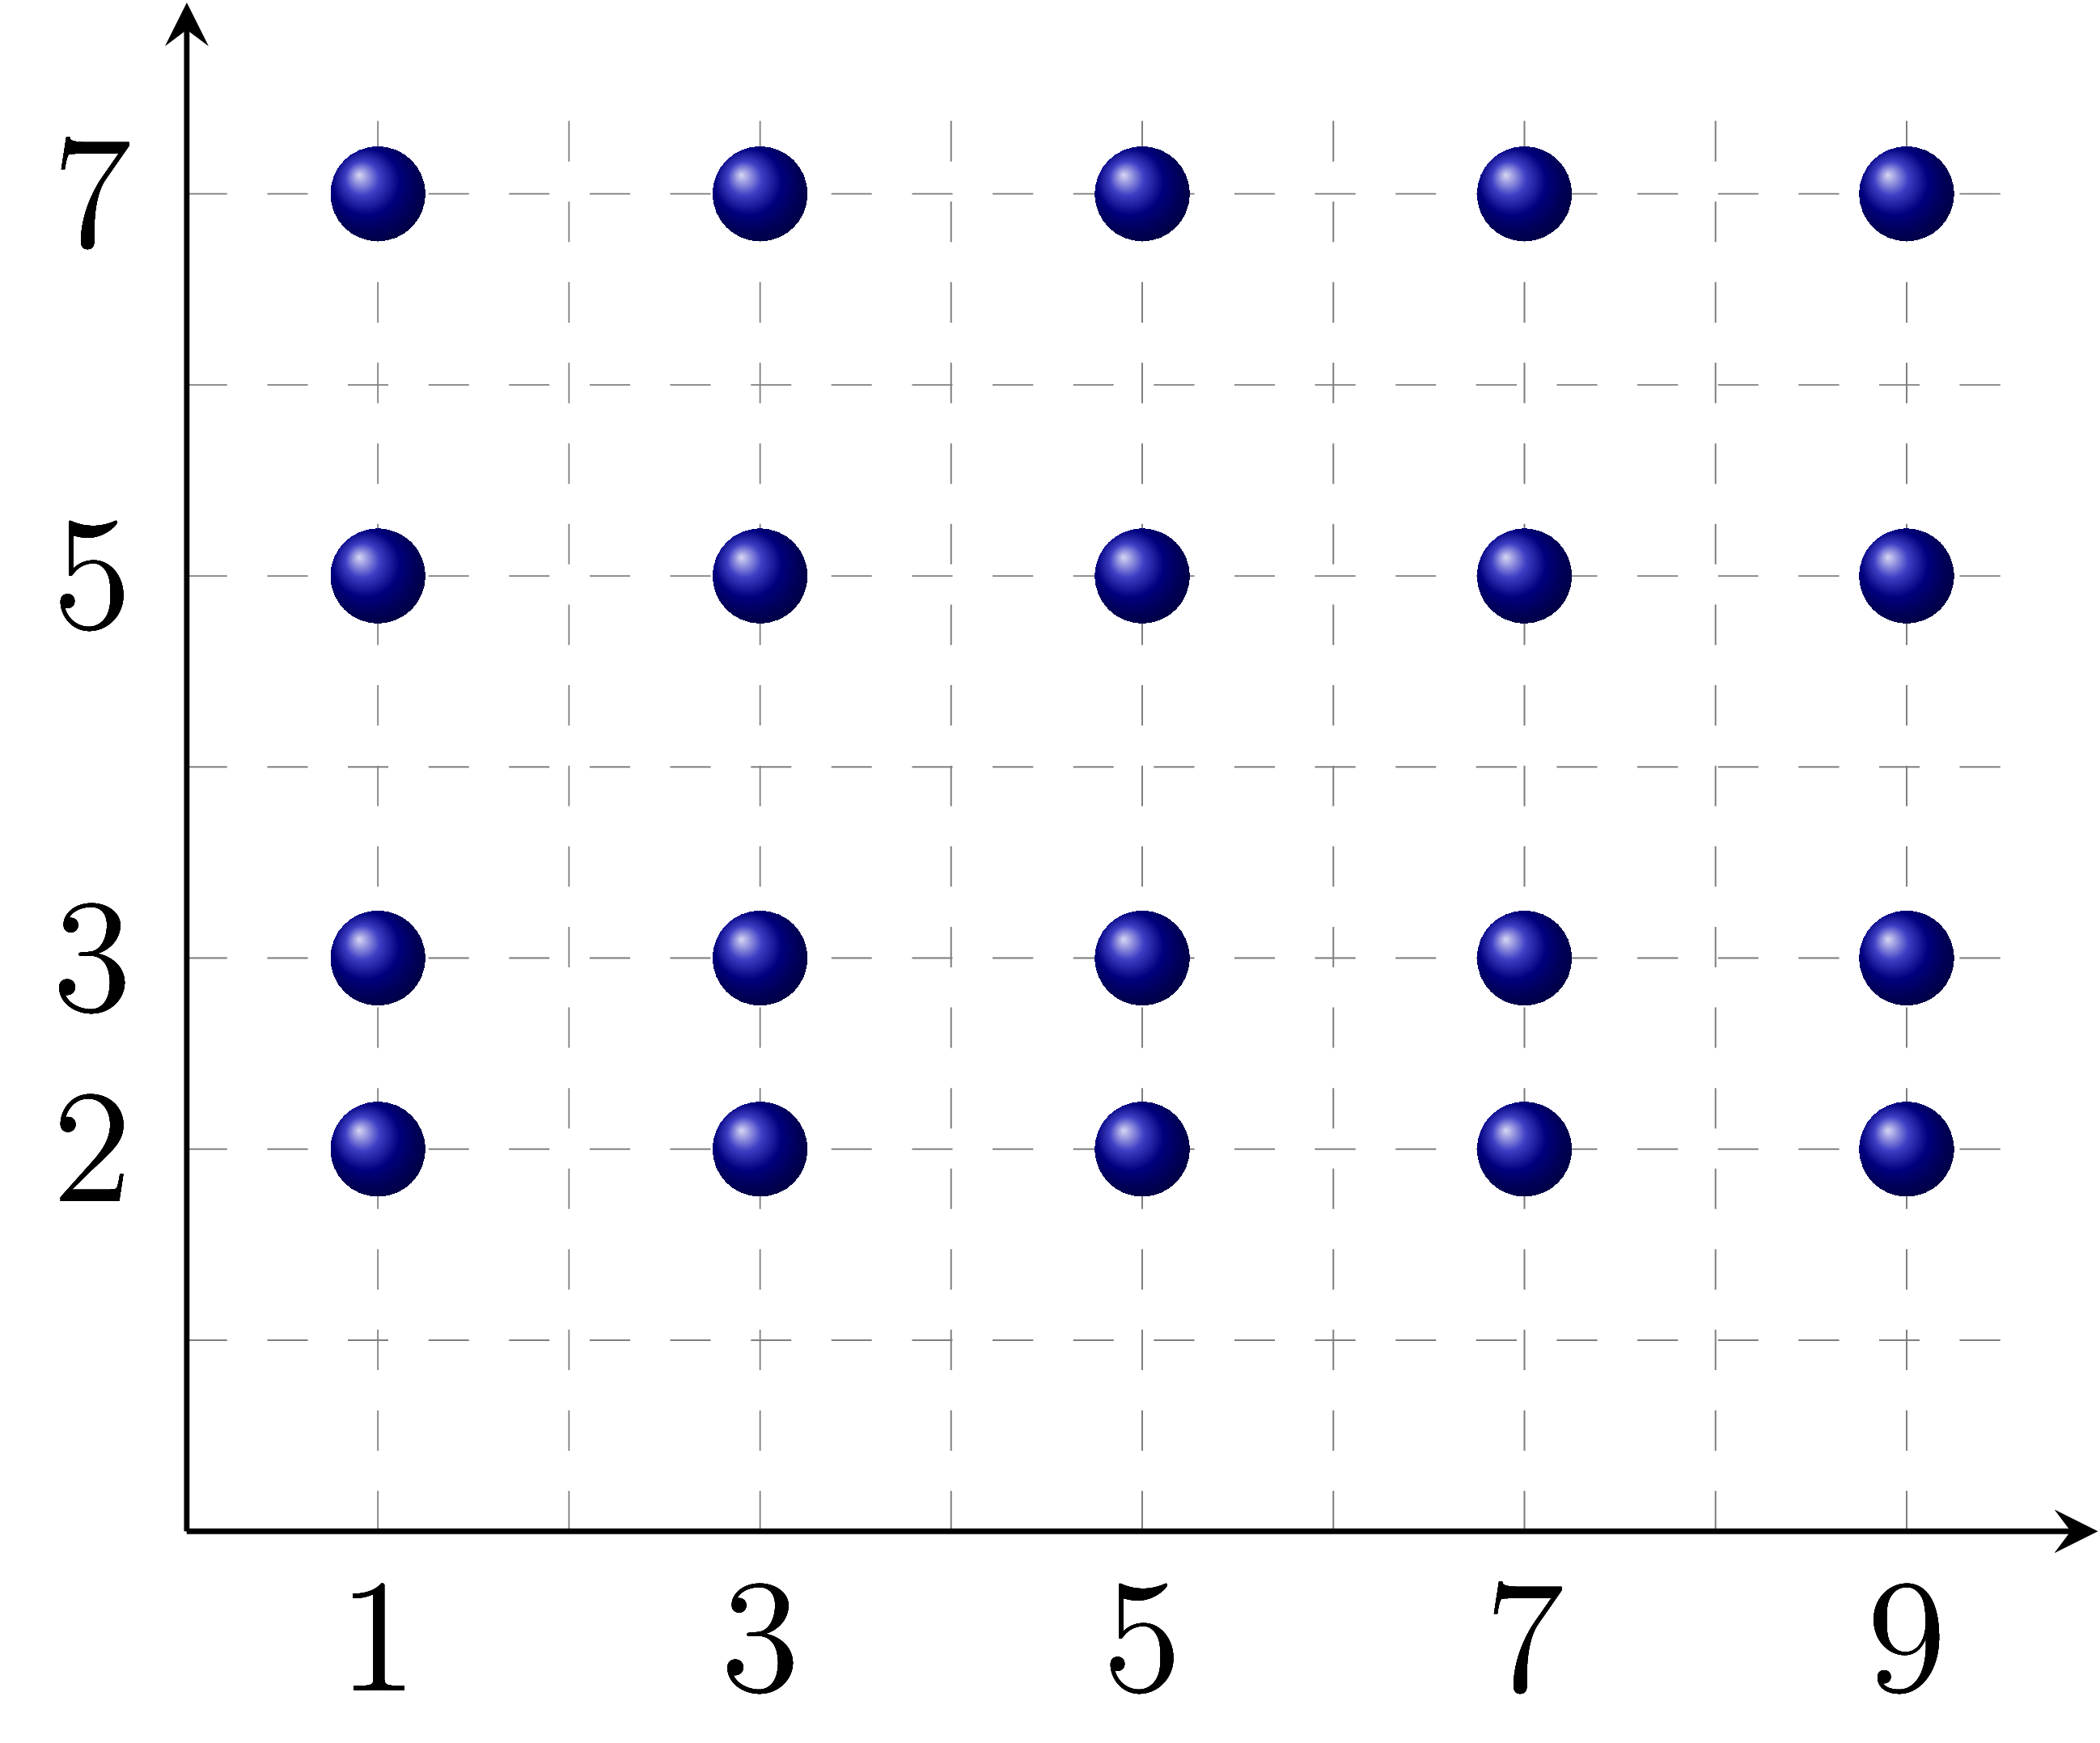
\includegraphics[scale=0.06,alt={Cartesian product of the sets A and B},width=0.35\linewidth]{images/created/cartesianproduct.png}
        \caption{Cartesian Product, \(A\times B\)}
        \label{fig:productvisualization}
    \end{figure}
\end{defn}

\clearpage

\begin{defn}[Subsets and Power Sets]\index{subset}\index{power set}
    A set \(X\) is a \emph{subset} of a set \(B\) if every element in \(X\) is also in \(B\), and we write
        \[X\subseteq B\ \text{if and only if}\ \forall x\in X: x\in B.\]
    
    With \(B=\left\{2,3,5,7\right\}\) we can use this to define the \emph{power set} of a set
    \begin{align}\label{eq:power_set}
        \mathscr{P}(B)&=\left\{\text{All the subsets of \(B\)}\right\}\\
            &=\left\{\emptyset,\{2\},\{3\},\{5\},\{7\},\{2,3\},\{2,5\},\{2,7\},\{3,5\},\{3,7\},\{5,7\}\right.\nonumber\\
            &\hspace*{24pt}\left.\{2,3,5\},\{2,3,7\},\{2,5,7\},\{3,5,7\},\{2,3,5,7\}\right\}\nonumber,
    \end{align}
    which is a new set with sets as elements.

    \begin{figure}[H]
        \centering
        % \inputtikz{powersetinclusiondiagram}
        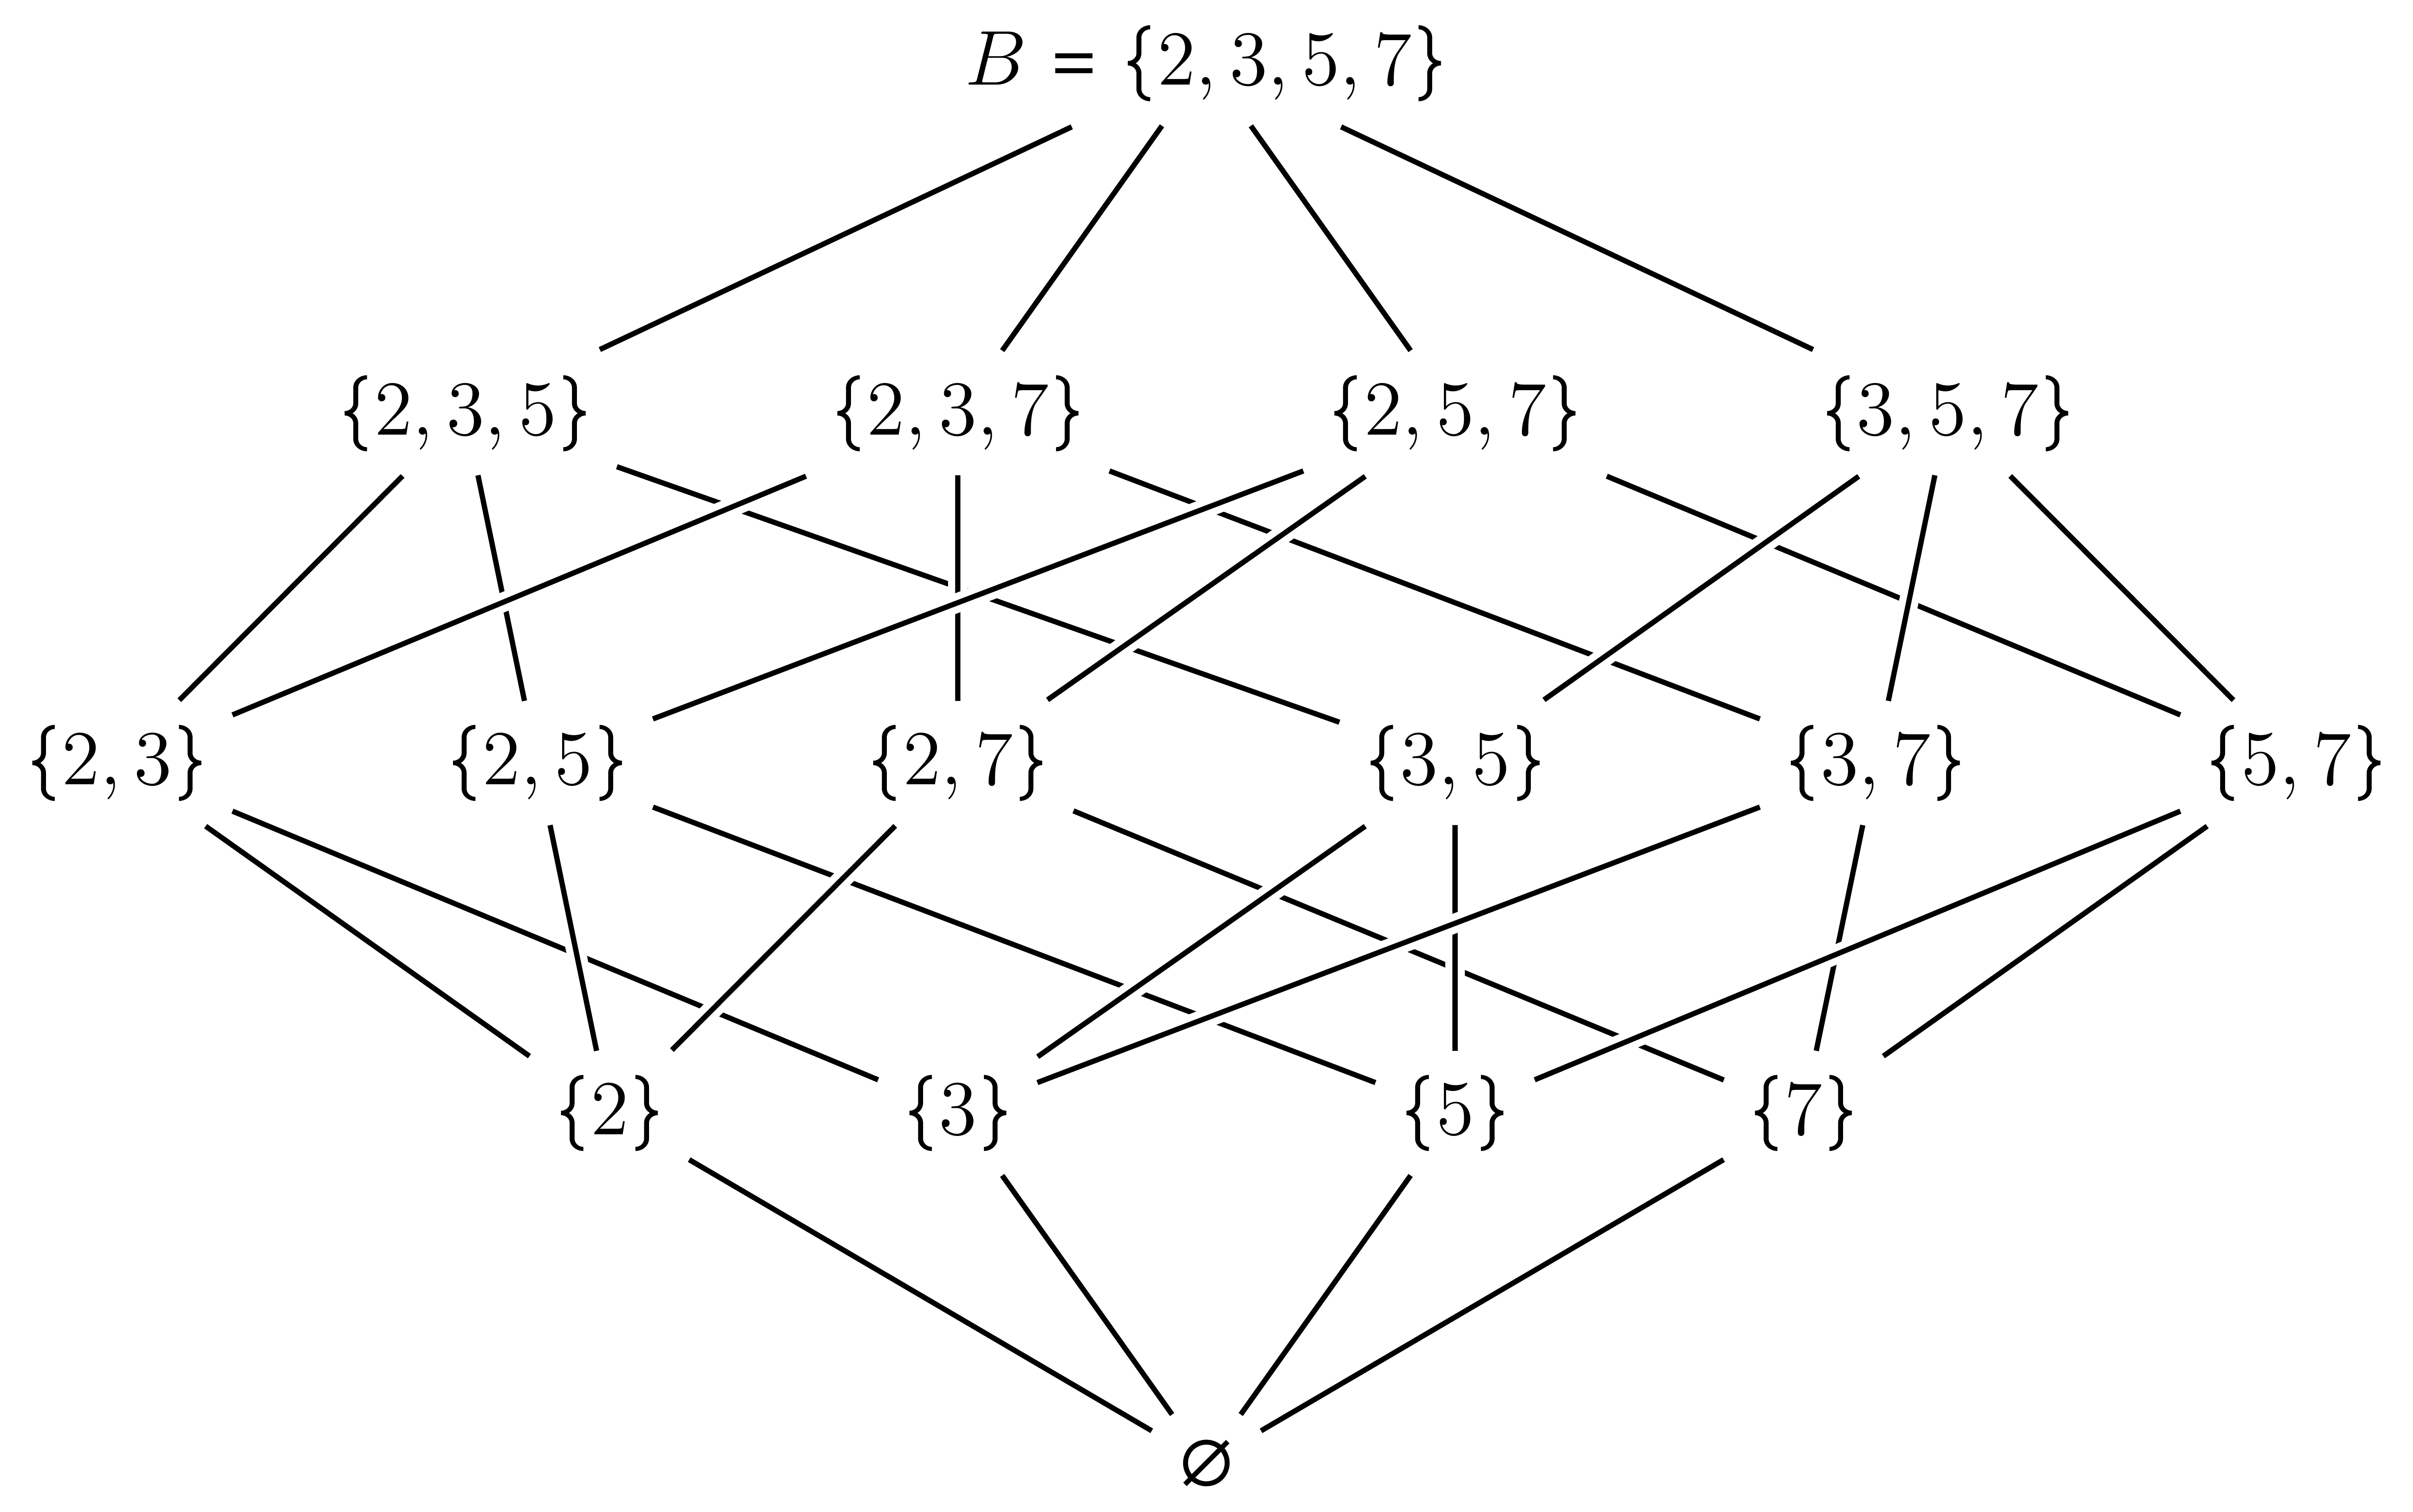
\includegraphics[scale=0.06,alt={Diagram of set inclusions in the power set of the set B},width=0.65\linewidth]{images/created/powersetinclusiondiagram.png}
        \caption{Set Inclusions in a Power Set}
        \label{fig:powersetinclusion}
    \end{figure}
\end{defn}

\begin{practiceprob}
    Use \(C=\{a,b,c\}\), \(D=\{a,b,c,d\}\), and \(N=\{1,2,3\}\) to fill in each of the following:
    \begin{align*}
        C\times N &= \left\{\phantom{\rule{0.85\textwidth}{10pt}}\right\}\\
        N\times C &= \left\{\phantom{\rule{0.85\textwidth}{10pt}}\right\}\\
        \mathscr{P}(C) &= \left\{\phantom{\rule{0.85\textwidth}{10pt}}\right\}\\
        \mathscr{P}(D) &= \left\{\phantom{\rule{0.85\textwidth}{10pt}}\right\}
    \end{align*}
    On a side note, what is the distinction between \(C=\left\{a,b,c\right\}\) and the set \(\left\{\{a\},\{b\},\{c\}\right\}\)?\vspace{30pt}
\end{practiceprob}

\begin{exposition}
    Look again at the power sets for \(C=\{a,b,c\}\) and \(D=\{a,b,c,d\}\).  How can we derive the power set for \(D\) starting with the power set for \(C\)?  How do they relate?  What does this tell us about the size of one compared to the other?
    \vspace{0.8\textheight}
\end{exposition}
\begin{thm}[Sizes of Power Sets]
    Given a finite set \(X\) with \(n\) elements, the size (\emph{cardinality}) of the power set of \(X\), \(\mathscr{P}(X)\), is equal to \(2^n\), i.e. \(\left|\mathscr{P}(X)\right|=2^n\).\index{cardinality}\index{power set!cardinality of}
\end{thm}



